%\documentclass{llncs}
%
\usepackage{makeidx}  % allows for indexgeneration
\usepackage{graphicx}
\usepackage{listings}
\usepackage{epsfig}
\usepackage[all]{xy}
%\usepackage{trackchanges}
%\renewcommand{\initialsOne}{RBA}
%
\begin{document}
\lstset{language=Haskell, numbers=left,
numberstyle=\tiny,numbersep=5pt,basicstyle=\scriptsize,aboveskip=20pt}
%
\frontmatter          % for the preliminaries
%
\pagestyle{headings}  % switches on printing of running heads
\addtocmark{Hamiltonian Mechanics} % additional mark in the TOC

\mainmatter              % start of the contributions

\title{Scenario Variability as Crosscutting}
%
\titlerunning{Requirement Variability as Crosscutting}  % abbreviated title (for running head)
%                                     also used for the TOC unless
%                                     \toctitle is used
%
\author{Rodrigo Bonif\'{a}cio \and Paulo Borba}
%
\authorrunning{Rodrigo Bonif\'{a}cio et al.}   % abbreviated author list (for running head)
%
%%%% modified list of authors for the TOC (add the affiliations)
\tocauthor{Rodrigo Bonifacio, Paulo Borba (Federal University of Pernambuco)}
%
\institute{Informatics Center \\ Federal University of Pernambuco \\ Recife, Brazil \\
\email{\{rba2,phmb\}@cin.ufpe.br},\\ WWW home page:
\texttt{http://www.cin.ufpe.br}
}

\maketitle              % typeset the title of the contribution

\begin{abstract}
Variability management is a common challenge for Software Product
Line (SPL) adoption. Developers need suitable
mechanisms for describing or implementing different kinds of variability
that might occurs at different SPL views (requirements, design,
implementation, and test). In this paper, we present a framework for
modeling use case scenario variability mechanisms, enabling better
separation of concerns between languages used to manage
variabilities and languages used to specify use case scenarios. The
result is that both representations can be understood and evolved in
a separated way. We achieve such goal by modeling variability management
as a crosscutting phenomenon, since features often affect
different points of each SPL view. Additionally, we believe that our proposed framework might be customized to 
describe variability mechanisms in other SPL artifacts, being a contribution for automatic product generation and traceability.
\end{abstract}
%
\section{Introduction}
%
The support for variation points enables product
customization from a set of reusable
assets~\cite{phol-spl-book}. However, variability management, due to
its inherent crosscutting nature, is a common challenge in software
product line (SPL) adoption~\cite{northrop-spl-book,phol-spl-book}.
Such crosscutting characteristic is materialized whenever a feature
requires variation points to be spread in different SPL artifacts. Actually, 
the representation of a variant feature is often spread not only 
in several artifacts, but also at the different product line views (requirements, 
design, implementation, and test). In this case, variability management, in 
the same way as the feature model and the architecture, represents a central concern in the SPL 
development and should not be tangled with existing artifacts~\cite{phol-spl-book}.   

However, current techniques for scenario variability 
management~\cite{favaro-icsr-98,bertolino-esec-2003,eriksson-splc-2005} do 
not present a clear separation related to the role of each involved language. 
The result is that variability mechanisms become tangled with scenario specifications. 
An example of this problem occurs when a scenario specification describes all possible variants. 
If one variant is removed from the product line, it would be necessary to change all related scenarios. 
In summary, it is difficult to evolve both representations. 

Another problem is the lack of a formal representation of the composition processes used 
to derive product specific scenarios. This is not suitable for current SPL generative 
practices; following the aforementioned works, it is difficult to automatically derive 
the requirements of a specific SPL member.  Although  the semantic composition of PLUC (Product 
Line Use Case)~\cite{bertolino-esec-2003} is defined in~\cite{fantechi-splc-2004}, such approach 
does not separate scenario specification from variability management. In order to explain in more details 
the problems addressed by this work, a motivating example is presented  in Section~\ref{sec:example}.  

In this paper, we describe a framework for modeling the composition 
process of scenario variabilities (Section~\ref{sec:models}). 
Such framework aims to: (1) represent a clear separation between variability management 
and scenario specification; and (2) specify how to weave these representations in order to generate
specific scenarios for a SPL member. The main contributions of this work are:

\begin{itemize}

\item Characterization of variability management as a crosscutting concern and, in this way, enforce that it  
must be represented as an independent view of the SPL. Although this work focus on requirement artifacts, 
more specifically use case scenarios, we argue that such separation is also valid for other SPL views.
  
\item A framework for modeling the composition process of scenario variability mechanisms. 
This framework gives a basis for describing variability mechanisms, 
allowing a better understanding of each mechanism. In this work, such framework is used for modeling 
the semantics of scenario variation mechanisms, but it might be customized for other SPL views.

\item Describe three scenario variation mechanisms using the
modeling framework. Such descriptions present
a more formal representation when compared to existing works; this is an
important property for supporting the automatic derivation of product
specific artifacts.
\end{itemize}

We evaluate our approach (Section~\ref{sec:analysis}) by comparing it 
to existing works and observing a set of three criteria: support for the 
different kinds of variability, separation of concerns, and design expressiveness.  We 
also relate our work with other research topics (Section~\ref{sec:related}) and present our concluding 
remarks in Section~\ref{sec:conclusions}.

%-----------------------------------------------------------------------
% Subsection: Motivating example
%-----------------------------------------------------------------------
\section{Motivating Example}
\label{sec:example}

In order to customize specific products, by selecting a valid feature configuration, variant points must be represented in the 
product line artifacts. Several variant notations have been proposed for use case scenarios, like Product Line Use Case Modeling for Systems and 
Software Engineering (PLUSS)~\cite{eriksson-splc-2005} and Product Line Use Cases (PLUC)~\cite{bertolino-esec-2003}. However, besides
the benefits of variability support, existing works do not present a clear separation between variability 
management and scenario specifications. In this section we illustrate the resulting problems using the \emph{eShop Product Line}~\cite{eshop-url} 
as a motivating example. 

The main use cases of the \emph{eShop Product Line} (EPL) 
allow the user to \emph{Register as a Customer}, \emph{Search for Products}, 
and \emph{Buy Products}.  Five variant features are described in the original specification,
allowing a total  of 72 applications to be derived from the product line~\cite{eshop-url}. Here, 
we consider extra features, such as \emph{Update User Preferences} that, based on the user historical data of searches 
and purchases, updates user preferences. Figure~\ref{fig:eshop-fm} presents part of the \emph{eShop} feature model, a 
domain artifact used for representing the common and variant features of a SPL~~\cite{gheyi-alloy-06,czarnecki-book,kang-foda-report}. 
As a brief introduction about the feature model notation, the relationships between a parent and its child are 
categorized as: \emph{Optional} (features that might not be select in a specific product), \emph{Mandatory} (feature that must be selected, if the parent is also 
selected), \emph{Or} (one or more subfeatures might be selected), and \emph{Alternative} (exactly one subfeature must be selected).     

 \begin{figure}[h]
 \begin{center}
  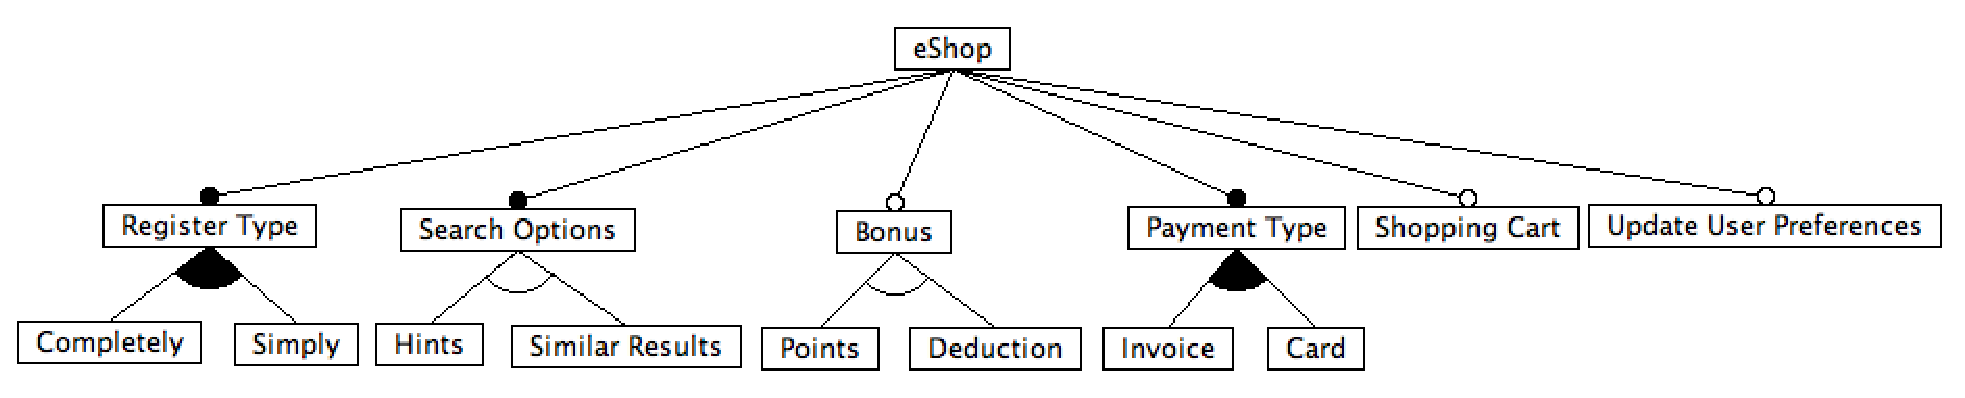
\includegraphics[scale=0.35]{img/eShop-fm3.eps}
   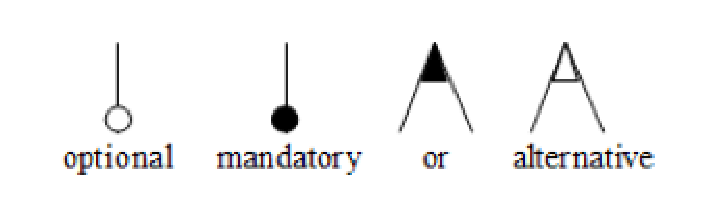
\includegraphics[scale=0.35]{img/fm-notation.eps}
  \caption{eShop feature model.}
  \label{fig:eshop-fm}
  \end{center}
\end{figure}


%Other approaches are based on use case extensions~\cite{jacobson-reuse-book}, not explored here since they 
%require that one use case extension must be defined for each variant. This can result in a huge
%number of use cases that is not suitable for managing activities.

In the PLUSS approach, all variant steps of a scenario specification are defined in the same artifact. For example, steps 1(a) and 1(b) in Figure ~\ref{fig:pluss-01} are 
never performed together. They are alternative steps: step 1(a) will be present only if the \emph{Shopping Cart} feature is selected (otherwise step 1(b) will be present). In a similar way, we have to choose between options (a) and (b) for step 2 (depending on the \emph{Bonus Feature} has been selected or not). Finally, step 6 is optional and will be present only if the feature \emph{Update User Preference} is selected. Following this approach, it is hard to understand a specific configuration because all possible variants are described in the same artifact. Also, such tangling between variant representation and scenario specification results in maintainability issues: introducing a new product variant might require changes in several points of existing artifacts.  For example, including a \emph{B2B Integration} feature, which allows the integration between partners in order to share their warehouses, might change the specification of \emph{Buy Product} scenario, enabling the search for product availability in remote warehouses (a new variant for step 1) and updating a remote warehouse when the user confirms the purchase (a new variant for step 5). Moreover, the inclusion of this new optional feature also changes the specification of \emph{Search for Products} scenario (the search might also be remote). 

Consequently, since the behavior of certain features can be spread among several specifications and each specification might describe several variants, the efforts needed to understand and evolve the product line might increase.    

\begin{figure}
\begin{center}
\begin{scriptsize}
  \texttt{
  \begin{tabular}{|p{0.3in}|p{2.2in}|p{2.2in}|}
   \hline
	Id    & User Action & System Response \\ \hline \hline    
       1(a) &Select the checkout option. & Present the items in the shopping cart and the amount to be paid. The user can remove items from shopping cart. \\  \hline
       1(b) & Select the buy product option. & Present the selected product. The user can change the quantity of item that he wants to buy. Calculate and show the amount to be paid. \\  \hline
       2(a) & Select the confirm option. & Request bonus and payment information. \\  \hline
       2(b) & Select the confirm option. & Request payment information. \\  \hline
       3     & Fill in the requested information and select the proceed option. & Request the shipping method and address.\\  \hline
       4     & Select the \$ShipMethod\$, fill in the destination address and select the proceed option. & Calculate the shipping costs. \\  \hline
       5     & Confirm the purchase. & Execute the order and send a request to the Delivery System in order to dispatch the products. \\  \hline
       6     & Select the close section option. & Register the user preferences.\\  \hline
  \end{tabular}
  } 
\end{scriptsize}
\caption{Buy Products scenarios using the PLUSS notation.}
\label{fig:pluss-01}
\end{center}
\end{figure}
  
Instead of relating each variant step to a feature, PLUC introduces special tags for representing 
variabilities in use case scenarios. For example, the VP1 tag in Figure~\ref{fig:pluc-01}, which also 
describes the \emph{Buy Products} scenario, denotes a variation point that might assumes the 
values ``\emph{checkout}'' or ``\emph{buy item}'', depending on which product was configured. For 
each \emph{alternative} or \emph{optional} step, one tag must be defined. The actual value
of each tag is specified in the \emph{Variation Points} section of the scenario specification. Another kind 
of tangling occurs in this case, since segments of the specification are tangled with the variation 
points. Additionally, SPL members are also described using the same tag notation (see the \emph{Product Definition} section 
in Figure~\ref{fig:pluc-01}). There is no explicit relationship between product configurations and feature models. In the example, 
two products (P1 and P2) are defined. The first product is implicitly configured by selecting the \emph{Shopping Cart}, 
\emph{Bonus}, and \emph{Update User Preferences} features. The second model, instead, is not configured 
with such features. Since the values of alternative and optional variation points are computed based on the defined products, instead 
of specific feature, the inclusion of a new member in the product line might require a deeply review of 
variation points. Moreover, since the variation points and the product definitions are spread among several scenario specifications, it is 
hard and time consuming keep the SPL consistent. Finally, the same definitions (product configuration and variation points) often are 
useful to manage variabilities in other artifacts, such as design and source code. As a consequence, this approach requires the replication of such 
definitions in different SPL views - if the SPL evolved, changes would be propagated throughout many artifacts.

\begin{figure}[t]
\begin{center}
\begin{scriptsize}
\fbox{
  \texttt{
  \begin{tabular}{l}
  {\bf Buy Products Scenario} \\
  {\bf Main Flow} \\
  01 Select [VP1] option \\
  02 [VP2] \\
  03 Select the confirm option \\
  04 [VP3] \\
  05 Fill in the requested information and select the proceed option \\
  06 Request the shipping method and address \\
  07 Select the [VP4] shipping method, fill in the destination address and ... \\
  08 Calculate the shipping costs. \\ 
  09 Confirm the purchase. \\
  10 Execute the order and sends a request to the Delivery System in .... \\  
  11 Select the close section option. \\ 
  12 \{[VP5] Register the user preferences.\} \\  \\
  {\bf Products definition: } \\ VP0 = (P1, P2) \\ \\
  {\bf Variation points: } \\ 
   VP1 =  if (VP0 == P1) then (checkout) else (buy product) \\
   VP2 =  if (VP0 == P1) \\ \hspace{0.25in}  then (Presents the items in the shopping cart...) \\ \hspace{0.25in} else (Present the selected product. The user can...) \\
   VP3 =  if (VP0 == P1) \\ \hspace{0.25in} then ( Requests bonus and payment information.) \\ \hspace{0.25in} else (Requests payment information.) \\
   VP4 =  (Economic, Fast) \\
   VP5 requires (VP0 == P1) \\
   \end{tabular}
  } }
\end{scriptsize}
\end{center}
\caption{Buy Products scenarios using the PLUC notation.}
\label{fig:pluc-01}

\end{figure}

In summary, both techniques rely on simple composition techniques: filtering variant steps in scenarios or syntactic changes of tag values based on product definition. In this sense, they are similar to conditional compilation techniques, which have been applied to implement variability at source code. Such techniques are not suitable for modularizing the crosscutting nature of certain features, has poor legibility and leads to lower maintainability~\cite{alves-gpce-06}. 
As a consequence, we argue that the variability management concern should be separated from the other artifacts and used as a language for generating specific products. The automatic generation of specific product artifacts has being recommended by the SPL community~\cite{krueger-cacm-200712,greenfield-softwarefactories,czarnecki-book}, in such way that the combination of generative techniques, aspect oriented programming, and software product line should be further investigated. In this case, in order to support the automatically derivation of product specific artifacts, it is necessary not only a more precise definition of each language used to describe product line artifacts and the variability management concern, but also the weave processes used to combine them. PLUSS and PLUC approaches fail in this direction, since Eriksson et al., although present the metamodel of PLUSS notation~\cite{eriksson-splc-2005}, do not describe which languages and processes are used for relating use case scenarios to feature models. Likewise, besides Fantechi et al. describe the formal semantics of PLUC~\cite{fantechi-splc-2004}, this approach does not separate variability management from use case scenarios.

The next section describes our approach that considers scenario variability as a composition of different artifacts. Although in this paper we are focus on use case scenarios, the idea of separating product line artifacts from variability management is also applied to other SPL views. Moreover, we believe that our modeling framework, which describes the weaving processes for handle variability management, might be customized for design, implementation, and test artifacts. 




%-------------------------------------------------------------------------
% Section: Scenario Variabilities
%------------------------------------------------------------------------
%\section{Scenario variabilities}
%\label{sec:req-var}

%Eriksson et al.~\cite{eriksson-splc-2005} presented
%four kinds of variabilities in use case models for product
%families: (i) use cases might be included
%in a given product ({\bf optional use cases}), (ii) certain
%scenarios of an included use case might be excluded from a
%particular product ({\bf optional scenarios}), (iii) the flow of
%events within an included scenario might vary ({\bf changing
%scenarios}), and (iv) crosscutting requirements might affect several
%use cases on several levels ({\bf crosscutting variability}).

%In order to illustrate examples of such variabilities, consider a Message Application Product Line (MAPL) used to create, receive, and 
%manage different kinds of message (such as e-mail, short messages, and multimedia messages) for mobile 
%devices. Depending on the target device, a specific member of the product line is composed by specific use case/scenario 
%configurations. Figure~\ref{fig:fm-01} depicts part of the Message Application feature model~\cite{czarnecki-book, czarnecki-
%wsfactory-2005, 
%kang-foda-report}, used for representing possible configurations 
%of the product line. For a better understanding of the example, we briefly introduce some features of the MAPL. 

%\begin{description}
%\item[Message Application (FEA01):] The MAPL root feature. This feature requires that some use cases must be present in all 
%members of the product line, such as \emph{Create and Send a Message} and \emph{Receive and Save a new Message} use cases.

%\item[Message Type (FEA02):] Feature used to represent the different kinds of messages (\emph{email}, \emph{sms}, \emph{mms}) 
%that might be supported by a product line member. At least one kind of message must be selected. 

%\item[Folder Management (FEA03):] Feature used to configure the folder management capabilities. Two kinds of folder management 
%are supported: single and multiple folders. If a product is configured with multiple folder support, the subscriber will be able to select 
%the place
%where a received message should be saved. Otherwise, the message must be saved on a specific folder (\emph{inbox folder}). 
%Multiple folder management also requires a specific use case (\emph{Manage Multiple Folders} use case) to \emph{create}, \emph
%{rename} and \emph{remove} folders and \emph{move messages} between folders. Additionally, Folder Management feature can be 
%configured as \emph{basic} or \emph{extended} size  (support for storing 1000 or 1500 messages).

%\end{description}
%  
%Suppose that if the feature \emph{Multiple Folders} is selected, 
%an extended version of \emph{Receive and Save a new Message} scenario
%and the \emph{Manage Multiple Folders} use case will be present in
%the target product (the basic version of \emph{Save a Message}
%scenario will not be present). In the SPL terminology, a
%\emph{configuration knowledge} should be used for describing 
%relationships between features and software artifacts
%(Table~\ref{tab:ck-01} is a simplified representation of a
%configuration knowledge). The variability related to the
%\emph{Manage Multiple Folders} use case is an example of optional
%use case variability. On the other hand, the \emph{basic} and
%\emph{extended} versions of \emph{Receive and Save a new Message} scenario compose an example of changing scenario 
%variability.

%\begin{figure}[h]
% 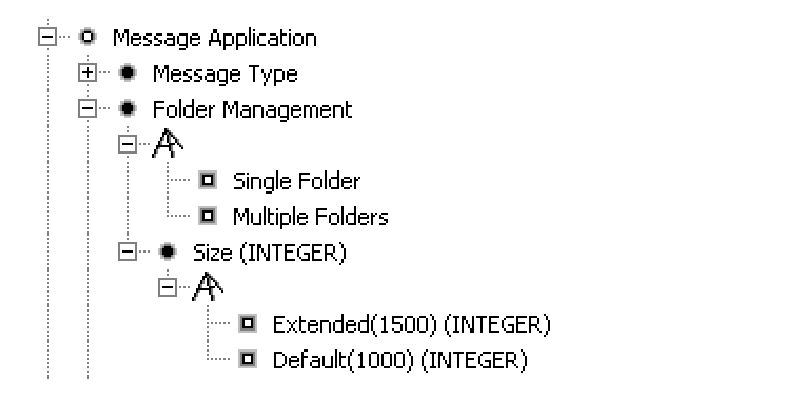
\includegraphics[scale=0.60]{img/fm03.eps}
%  \caption{Message Application feature model.}
%  \label{fig:fm-01}
%\end{figure}

%\begin{table}[h]
%\begin{tabular}{|l|l|}
%  \hline
%  {\bf Selected Feature} & {\bf Artifacts} \\ \hline \hline
%  Single Folder & Save Message (basic version) \\ \hline
%  Multiple Folders & Save Message (extended version) \\
%                   & Manage multiple folders use case \\
%  \hline
%\end{tabular}
%\caption{Folder management configuration.} \label{tab:ck-01}
%\end{table}

%Eriksson proposed the use of parameters in 
%order to describe crosscutting variabilities that change the behavior of different scenarios. 
%However, we believe that such kind of variability 
%should be described using quantification mechanisms, instead of parameters. In a previous work~\cite{gcabral-sbmf-2006}, the 
%quantification was achieved by enumerating all 
%the \emph{previous} and \emph{next steps} that delimits the starting and ending points of a given
%scenario (below we present our definition for scenario specification, 
%adapted from~\cite{gcabral-sbmf-2006}).

%\begin{description}
%\item[Scenario:] A use case scenario corresponds to a sequence of
%steps (a pair of \emph{User Action} x \emph{System Response}).
%Depending on the user action or system state, the behavior of a
%scenario can be changed. A use case defines a set of scenarios; and a use case model, 
%instead, defines a set of use cases.
%\end{description}

%In order to enable a better modularity (see figures~\ref{fig:pm-01} and~\ref{fig:alt-01}), a
%scenario could be \emph{started} from steps of different scenarios
%(using the \emph{from step} clause) and \emph{finished} by steps of
%other scenarios (using the \emph{to step} clause). Following the same 
%example of message application, two alternative flows are presented in Figure~\ref{fig:alt-01}. The first scenario,
%that allows a subscriber to save an edited message, changes the
%behavior of \emph{Create and Send a Message Scenario} (Figure~\ref{fig:pm-01})
%from \emph{Step 5M} to the \emph{end} of execution (see the
%\emph{from} and \emph{to step} clauses). The second one, instead, is
%an exception flow that describes the phone behavior when the
%subscriber tries to send or save a message and the message box is
%full. Such scenario changes the behavior of \emph{Create and Send a Message
%Scenario} (from \emph{Step 7M}) and \emph{Save a Message to Draft Folder Scenario}
%(from \emph{Step A1.1}). Such exception flow is an example of crosscutting
%variability, since it changes the behavior of multiple scenarios.

%Previously, only explicit references to the step ids (eg.: 5M, 7M,
%A1.1) are allowed in the \emph{from step} and \emph{to step}
%clauses~\cite{gcabral-sbmf-2006}. Therefore, the weaving rules of
%two or more scenarios are basically
%syntactic~\cite{rashid-aosd-2007}, resulting in \emph{fragile
%pointcuts} (a scenario composition could break, if we change a step
%id). In order to solve this problem, the use of semantic scenario
%compositions, based on the meaning of natural language
%specifications, was proposed by Rashid et
%al.~\cite{rashid-aosd-2007}. 

%In this paper, we propose a more simplistic semantic composition based on the use of annotations. We enrich scenario specifications 
%allowing a step to be marked with zero or more annotations; and the \emph{from steps} and \emph{to
%steps} clauses referring to steps in other scenarios by \emph{step ids}
%or by \emph{annotations}.

%
%\begin{figure}[h]
%%  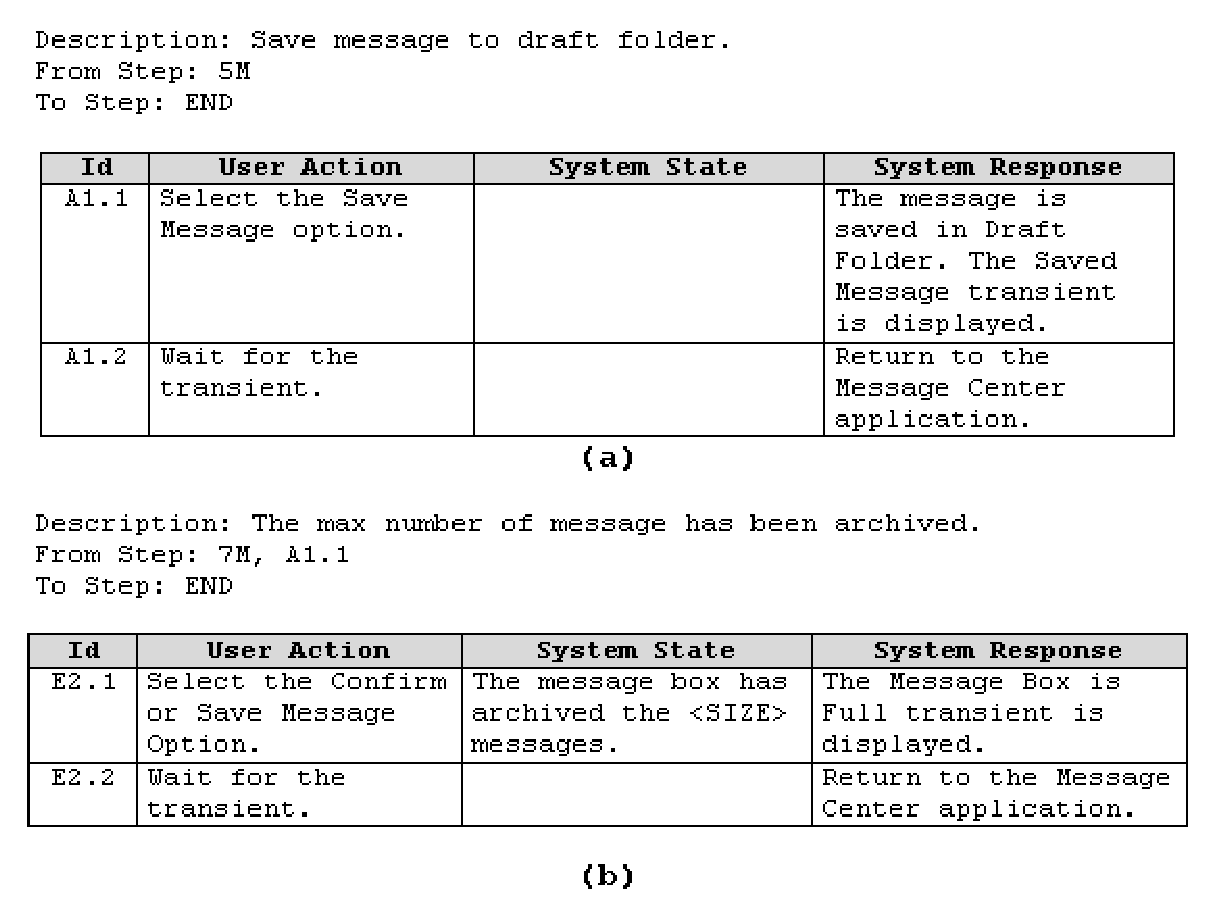
\includegraphics[scale=0.45]{img/alternative01.eps}
%  \begin{scriptsize} 
%  \texttt{
%  \begin{tabular}{l}
%  {\bf Basic Flow}\\
%  Description: Create and send a message.\\
%  From step: START\\
%  To Step: END\\
%  \end{tabular}  
%  \begin{tabular}{|p{0.2in}|p{0.8in}|p{0.8in}|p{1in}|}
%   \hline
%	Id & User Action & System State &  System Response \\ \hline \hline    
%	... & ... & ... & ... \\ \hline
%	3M  & Select a \mbox{<MessageType>} from the create message men.u & & The Create a New <MessageType> form is 
%displayed. \\ \hline
%	4M  & Fill the message body. & & The message body is filled. \\ \hline
%	5M  & Select the send message option. & The message body is not empty & The Recipient form is displayed. \\ \hline
%	6M  & Fill the recipient field. &  & The Recipient field is filled. \\ \hline
%	7M  & Select the confirm option. & The message box has not reached <Size> messages.  & The message is sent to the recipient 
%and saved in Sent Items folder. The Sent Message transient is displayed. \\ \hline 
%	... & ... & ... & ... \\ \hline
%  \end{tabular} 
%  }
%  \end{scriptsize}
%  \caption{Create and Send a Message scenario.}
%  \label{fig:pm-01}
%\end{figure}

%\begin{figure}[t]
%  \begin{scriptsize} 
%  \texttt{
%  \begin{tabular}{l}
%  Description: Save a message to draft folder\\
%  From step: 5M\\
%  To Step: END\\
%  \end{tabular}  
%  \begin{tabular}{|p{0.2in}|p{0.8in}|p{0.8in}|p{1in}|}
%   \hline
%	Id & User Action & System State &  System Response \\ \hline \hline    
%	A1.1 & Select the save message option. & There is enough space to save the message. &  The message is saved in draft folder. 
%The saved message transient is displayed. \\ \hline
%	A1.2 & Wait for the transient. & & Return to the Message Center Application.
%   \\ \hline
%  \end{tabular} 
%  }
%  \end{scriptsize}
%  \center{(a)}
%  
%  \begin{scriptsize} 
%  \texttt{
%  \begin{tabular}{l}
%  Description: The maximum number of messages has been achieved\\
%  From step: 7M, A1.1\\
%  To Step: END\\
%  \end{tabular}  
%  \begin{tabular}{|p{0.2in}|p{0.8in}|p{0.8in}|p{1in}|}
%   \hline
%	Id & User Action & System State &  System Response \\ \hline \hline    
%	E2.1 & Select the confirm or save message option. & Message box has achieved the <SIZE> messages. &  The Message Box is 
%Full transient is displayed. \\ \hline
%	E.2.2 & Wait for the transient. & & Return to the Message Center Application.
%   \\ \hline
%  \end{tabular} 
%  }
%  \end{scriptsize}
%  \center{(b)}
%  \caption{Send a Message alternative flows.}
%  \label{fig:alt-01}
%\end{figure}

%A final remark related to the scenario variability taxonomy is that we are proposing a new kind of variability: one that represents 
%parametric scenario specifications. Such kind of variability occurs whenever two similar behaviors vary only in accordance with 
%parameterized values. For example, Figure~\ref{fig:pm-01} depicts a scenario specification for \emph{sending a message} using 
%parameters  for reuse it with different \emph{kinds of message} (\emph{MessageType} parameter on step 3M) and \emph{message 
%folder sizes} (\emph{Size} parameter on step 7M). Parametric scenarios increase the requirement coverage and avoid duplicated 
%scenario specifications. Notice that the domain values for those parameters are defined in the feature model (features \emph
%{MessageType} and
%\emph{Size} in Figure~\ref{fig:fm-01}). In this way, the \emph{MessageType}
%parameter of step 3M abstracts over the different kinds of messages (\emph{email}, \emph{sms}, and \emph{mms}); and the  \emph
%{Size} parameter of step 7M abstracts over the values \emph{extended folder size} and \emph{default folder size} (Figure~\ref
%{fig:fm-01}).


%-------------------------------------------------------------------------
% Section: Modeling the Variability Mechanisms
%------------------------------------------------------------------------
\section{Scenario Variability as Crosscutting}
\label{sec:models}

Aiming to represent a clear separation between variability management and scenario specification, and also 
describe the weave processes required to compose those views, we are proposing a modeling framework that is a 
customization of the Masuhara and Kiczales (MK) work~\cite{kiczales-ecoop-2003}. The goal of MK framework is to
explain how different \emph{aspect-oriented} technologies support crosscutting modularity. Each technology is modeled 
as a three-part description: the related weave processes take two programs as input, which crosscut each other with respect 
to the resulting program or computation~\cite{kiczales-ecoop-2003}. 

Similarly to the MK framework, we represent the semantics of \textbf{scenario variability management} as a weaver that takes four specifications
as input (\emph{product line use case model}, \emph{feature model}, \emph{product configuration}, and \emph{configuration knowledge}) that 
crosscut each other with respect to the resulting product specific use case model (Figure~\ref{fig:weave-process}). Combining these input languages, 
it is possible to represent the kinds of variability that we are interest in: \emph{optional use cases and scenarios}, \emph{quantified changed scenarios}, 
and \emph{parameterized} scenarios. 

A running example of our approach is presented in Section~\ref{sub:running}. After, we describe the semantics of our weaving process. For 
simplicity, it was decomposed in three subcomponents - one weaver process for each kind of variability.  The semantics of those 
weavers (and the meta-model of the input and output languages) are described using the Haskell programming language~\cite{haskell-report}. 
Such decision allows the execution and testing of concise weaving processes descriptions (all related source code is available at 
SPG web site~\cite{spg-url}).

%\begin{figure}[h]
% 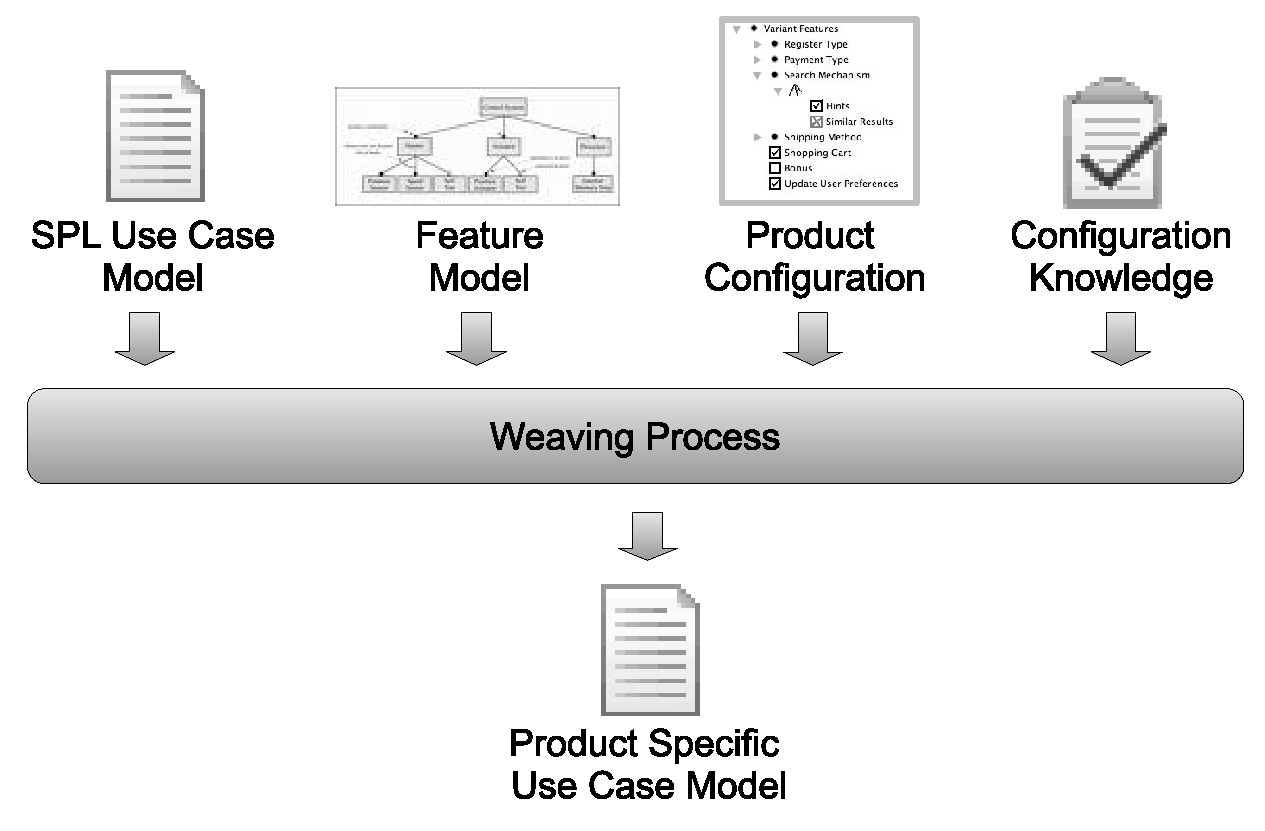
\epsfig{file=img/weave-process2.eps,scale=0.3}
% \caption{Overview of the modeling framework.}
% \label{fig:weave-process}
%\end{figure}

\begin{figure}[h]
 \begin{center}
  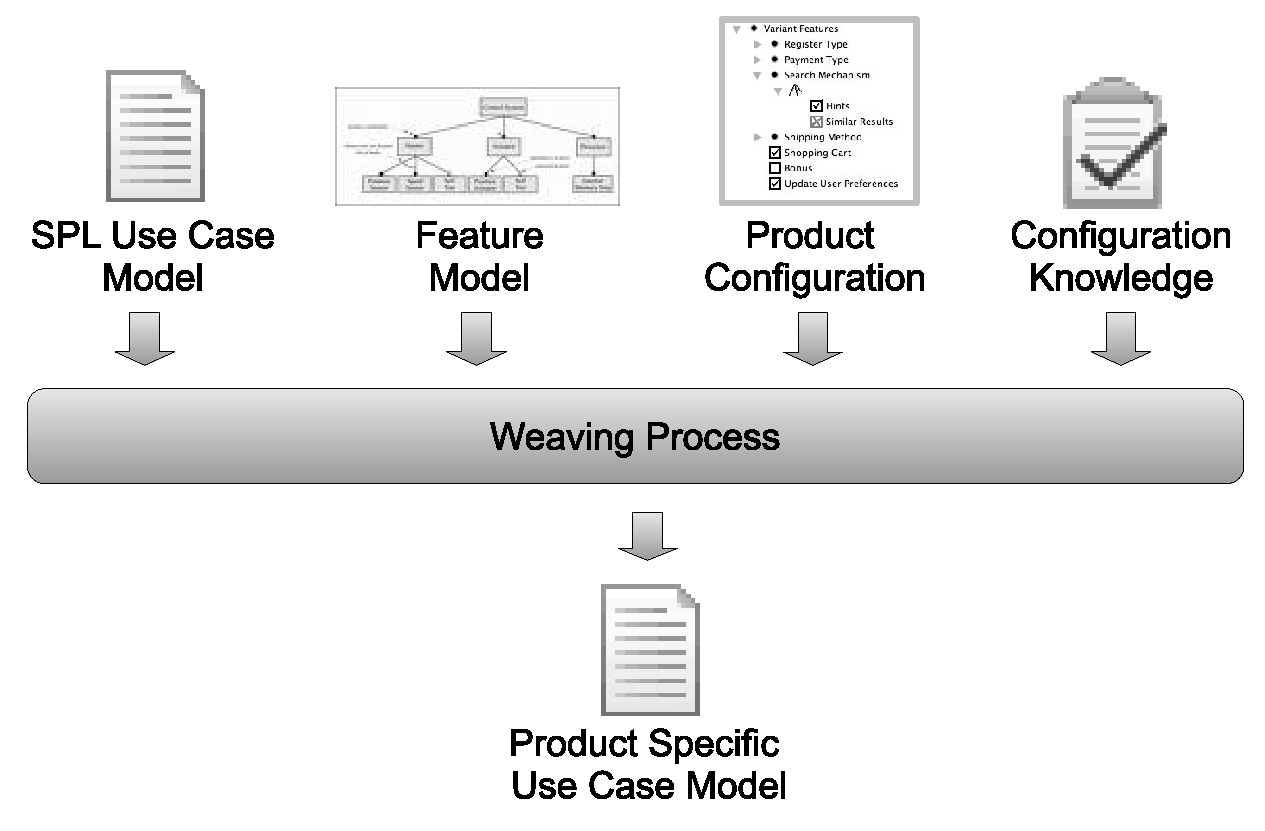
\includegraphics[scale=0.30]{img/weave-process2.eps}
  \caption{Overview of the modeling framework.}
  \label{fig:weave-process}
  \end{center}
\end{figure}

\subsection{Running example}
\label{sub:running}

In order to explain how the input languages crosscut each other and produce a product specific use case model, here we present a 
running example based on the eShop Product Line (briefly introduced in Section~\ref{sec:example}). For this, several artifacts of each 
input language are described. Then, we present the role of each input language in respect of the weaving process.

\subsubsection{SPL use case model:} 

defines a set of scenarios that might be used to describe possible variants of the product line. This artifact is not directly concerned 
with variability management, although some scenarios might be optional, might have parameters, or might change the behavior of other 
scenarios. Based on the notation proposed by~\cite{gcabral-sbmf-2006},  a use case scenario corresponds to a sequence of
steps (a tuple of \emph{User Action} x \emph{System State} x \emph{System Response}). Depending on the user action or system state, 
the behavior of a scenario can be changed. A use case defines a set of scenarios; and a use case model, instead, defines a set of use cases.
In this running example, we are considering the following scenarios:

\begin{enumerate}

\item {\bf Buy Item Basic Version:} this scenario (Figure~\ref{fig:buy-product-basic-flow}) specifies the basic behavior of \emph{Buy Products},
assembled in products that are not configured with the \emph{Shopping Cart} and \emph{Bonus} features. It starts from the IDDLE special state 
(do not extend the behavior of an existing scenario) and finishes at the END of execution (in this case, there is no other behavior to be performed).
The clauses \emph{From step} and \emph{To step} are used for describing the possible starting and ending points of execution.
 
\begin{figure}[h]
\begin{scriptsize}
  \texttt{
   \begin{tabular}{l}
     Description: Basic version of Buy Products scenario\\
     From step: IDDLE \\
     To step: END
   \end{tabular}  
  \begin{center} 
  \begin{tabular}{|p{0.3in}|p{1.4in}|p{1.4in}|p{1.4in}|}
   \hline
       Id    & User Action & System State & System Response \\ \hline \hline
       1M & Select the buy product option. & & Present the selected product. The user can change the quantity of item that he wants to buy. Calculate and show the amount to be paid. \\  \hline
       2M & Select the confirm option. & & Request payment information. \\  \hline
       3M & Fill in the requested information and select the proceed option. &  & Request the shipping method and address.\\  \hline
       4M & Select the <ShipMethod>, fill in the destination address and proceed. & & Calculate the shipping costs. \\  \hline
       5M & Confirm the purchase. & & Execute the order and send a request to the Delivery System to dispatch the products. [RegisterPreference] \\  \hline
  \end{tabular}
  \end{center}
  } 
\end{scriptsize}
\caption{Basic version of Buy Products scenario.}
\label{fig:buy-product-basic-flow}
\end{figure}

 Notice that a parameter \emph{ShipMethod} is referenced in step 4M of Figure~\ref{fig:buy-product-basic-flow}. The use of this parameter (notation also supported in PLUSS and PLUC) allows the reuse of this specification 
for different kinds of \emph{ship method} configurations.


\item {\bf Buy Products with Shopping Cart and Bonus:} this scenario (Figure~\ref{fig:buy-product-changing-flow}) changes the behavior of 
the \emph{Buy Products Basic Version} by replacing its first two steps, introducing the specific behavior required by the \emph{Shopping Cart} and 
\emph{Bonus} features. This scenario also starts from the IDDLE state (\emph{from step} clause), however, it returns to the third step of the \emph{Buy 
Products Basic Version} (\emph{to step} clause). This behavior is required for products that are configured with \emph{Shopping Cart} and \emph{Bonus} features.

\begin{figure}[h]
\begin{scriptsize}
  \texttt{
   \begin{tabular}{l}
     Description: Extended version of Buy Products scenario\\
     From step: IDDLE \\
     To step: 3M
   \end{tabular}  
  \begin{center} 
  \begin{tabular}{|p{0.3in}|p{1.4in}|p{1.4in}|p{1.4in}|}
   \hline
       Id & User Action & System State & System Response \\ \hline \hline
       V1 & Select the checkout option. & & Present the items in the shopping cart and the amount to be paid. The user can remove items from shopping cart. \\  \hline
       V2 & Select the confirm option. & & Request bonus and payment information. \\  \hline
  \end{tabular}
  \end{center}
  } 
\end{scriptsize}
\caption{Extended version of Buy Products scenario.}
\label{fig:buy-product-changing-flow}
\end{figure}

\item {\bf Search for Products:} this scenario allows the user to search for products. In order to save space, we are only presenting the step (3S) that 
perform a search based on the input criteria. This step is annotated with the mark \mbox{{\bf [RegisterPreference]}}, exposing it as a possible point that the 
behavior of \emph{Register User Preferences} might starts. The same annotation was used in the \emph{step 5M} of \emph{Buy Products Basic Version}. Such 
annotations can be referenced in the \emph{from step} and \emph{to step} clauses, reducing 
the problem of \emph{fragile pointcuts}~\cite{rashid-aosd-2007}.

\begin{figure}[h]
\begin{scriptsize}
  \texttt{
   \begin{tabular}{l}
     Description: Search for Products scenario\\
     From step: IDDLE \\
     To step: END
   \end{tabular}  
  \begin{center} 
  \begin{tabular}{|p{0.3in}|p{1.4in}|p{1.4in}|p{1.4in}|}
   \hline
       Id & User Action & System State & System Response \\ \hline \hline
       \ldots & \ldots & \ldots & \ldots \\  \hline
       3S & Inform the search criteria. & & Retrieve the products that satisfy the search criteria. Show a list with the resulting products. [RegisterPreference] \\  \hline
  \end{tabular}
  \end{center}
  } 
\end{scriptsize}
\caption{Search for Products scenario.}
\label{fig:search-products-flow}
\end{figure}

\item {\bf Register User Preferences:} this scenario updates the user preferences based on the buy and search products use cases. Its behavior can be 
started at each step that is marked with the {\bf [RegisterPreference]} (see the \emph{from step} clause) annotation and is available in products 
that are configured with the \emph{Register User Preferences} feature.

\begin{figure}[h]
\begin{scriptsize}
  \texttt{
   \begin{tabular}{l}
     Description: Register user preferences based on searches and purchases \\
     From step: [RegisterPreference] \\
     To step: END
   \end{tabular}  
  \begin{center} 
  \begin{tabular}{|p{0.3in}|p{1.4in}|p{1.4in}|p{1.4in}|}
   \hline
       Id & User Action & System State & System Response \\ \hline \hline
       1R & - & & Update the preferences based on the search results or purchased items. \\  \hline
  \end{tabular}
  \end{center}
  } 
\end{scriptsize}
\caption{Register user preferences based on searches and purchases}
\label{fig:search-products-flow}
\end{figure}

\end{enumerate}


\subsubsection{Feature model:}

we have introduced part of this artifact for the eShop product line in Section~\ref{sec:example}. However, here we are going to 
present only the features that are fundamental for the running example. Based on the feature model of Figure~\ref{fig:eshop-fm-re}, the \emph{Shopping 
Cart}, \emph{Bonus} and \emph{Update User Preferences} features are not required; on the other had, the feature \emph{Ship Method} is mandatory and 
a specific product might be configured with at least one of its child.  

 \begin{figure}[h]
 \begin{center}
  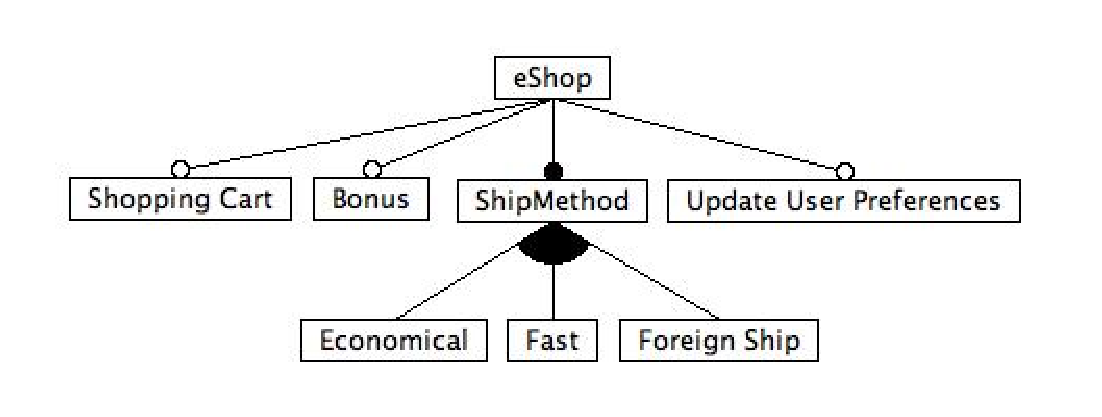
\includegraphics[scale=0.40]{img/eShop-fm-re.eps}
   \caption{eShop feature model for the running example.}
  \label{fig:eshop-fm-re}
  \end{center}
\end{figure}


\subsubsection{Product configuration:}

identifies which features were selected in order to compose a specific member of a product line. Each product configuration should 
conform to a feature model (the selected features should obeyed the feature model relationships and constraints). Two possible 
configurations are presented in Figure~\ref{fig:product-config-01-02}. The first configuration (on the left side of the figure) defines a
product that has no support for shopping cart, bonus and updating preferences. Additionally, it supports only the economical and fast 
ship methods. The second configuration selects all possible features.  

\begin{figure*}[h]
  \centerline{
    \mbox{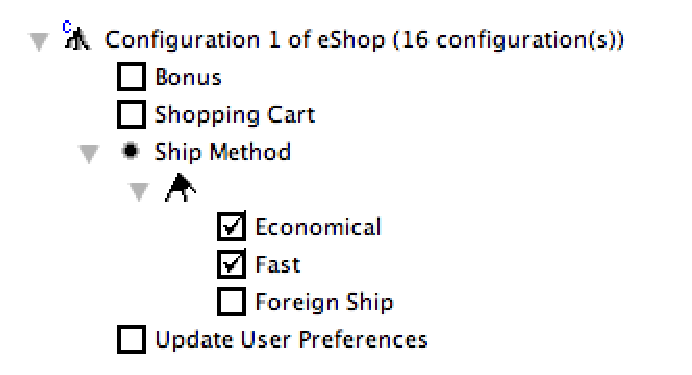
\includegraphics[scale=0.5]{img/pc-01.eps}}
    \mbox{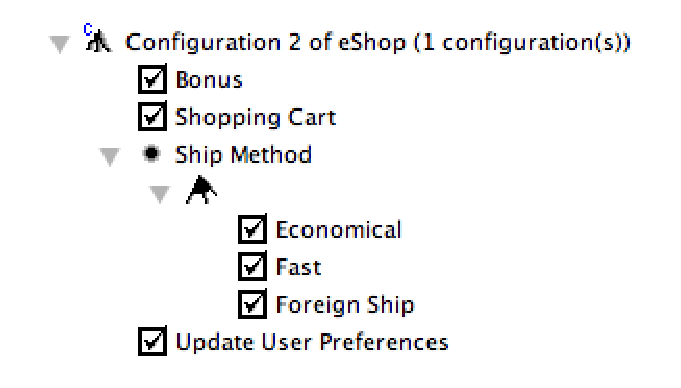
\includegraphics[scale=0.5]{img/pc-02.eps}}
  }
  \caption{Examples of product configurations.}
  \label{fig:product-config-01-02}
  \end{figure*}

\subsubsection{Configuration knowledge:}

relates feature expressions with artifacts that must be assembled in a given
product. Such artifact allows, during the product engineering phase, the automatically selection of assets that are 
required for a specific product configuration. Table~\ref{tab:eshop-running-example} presents a configuration knowledge 
for the running example, enforcing that: if \emph{Shopping Cart} and \emph{Bonus} features are {\bf not} selected, the 
basic version of \emph{Buy Product} scenario will be assembled; otherwise, the extended version of the same 
scenario will be assembled; and the \emph{Register User Preferences} scenario will be assembled only if the \emph{Update 
User Preferences} feature is selected.

\begin{table}[h]
\begin{center}
\caption{eShop configuration knowledge for the running example} \label{tab:eshop-running-example}
\begin{tabular}{ll}
   \hline\noalign{\smallskip}
  {\bf Expression} & {\bf Required Artifacts} \\
   \noalign{\smallskip}
   \hline
   \noalign{\smallskip}
    \ldots & \ldots \\
    {\bf not} (Shopping Cart {\bf and} Bonus)\hspace{2pt} & Basic version of Buy Products scenario \\
    Shopping Cart {\bf and} Bonus & Extended version of Buy Products scenario \\
    Update User Preferences & Register user preferences scenario	 \\       
  \hline
\end{tabular}
\end{center}
\end{table}

\subsubsection {Weaving process:} After presenting input artifacts for the running example, we are ready to describe the waving process that combine 
the input languages in order to derive product specific scenarios. In the next section we present, more precisely, the semantics of its components using a low level design. The weave process is composed by four activities, although the last one is optional: 

\begin{enumerate}
\item {\bf Validation:} This activity is responsible for checking if a product configuration is a valid instance of the feature model. If the product configuration is 
valid (it is conform to the relationship cardinalities and constraints of the feature model), the process might proceed. Otherwise, an error should be reported. In the running example, both configurations presented in Figure~\ref{fig:product-config-01-02} are valid. 

\item {\bf Product derivation:} This activity takes as input a (valid) product configuration and a configuration knowledge. Then, each feature expression of the 
configuration knowledge is checked against the product configuration. If the expression is satisfied, the related scenarios are assembled as the result of 
this activity. For the running example, Table~\ref{tab:assembled-scenarios} shows the assembled scenarios for the configurations in  
Figure~\ref{fig:product-config-01-02}.

\begin{table}[h]
\begin{center}
\caption{Assembled scenarios for each configurations of the running example} \label{tab:assembled-scenarios}
\begin{tabular}{ll}
   \hline\noalign{\smallskip}
  {\bf Configuration} & {\bf Assembled scenarios} \\
   \noalign{\smallskip}
   \hline
   \noalign{\smallskip}
    Configuration 1\hspace{15pt} & Basic version of Buy Products \\
                             & Search for products \\
                             & \ldots \\
   Configuration 2 & Extended version of Buy Products \\
                             & Search for Products	 \\
                             & Register user Preferences \\
                             & \ldots       \\
  \hline
\end{tabular}
\end{center}
\end{table}
 
 \item {\bf Scenario composition:} This activity is responsible for composing the scenarios assembled for a specific product configuration. 
 The resulting scenarios of the previous activity, which crosscut each other based on the \emph{from step} and \emph{to step clauses}, are waved. The 
 result is either a use case model with complete paths (all \emph{from step} and \emph{to step} clauses are resolved) or a trace model (a set of all valid sequences of events extracted from the complete paths). 
 
The complete path is a high level representation, which uses the same constructions of the use case model (scenarios), and can be represented using a graph notation, where each node is labeled with a step id. For example, Figure~\ref{fig:complete-paths} depicts the complete paths for the first and second configurations of our running example. In the left side of the figure,  the basic versions of search for product (branch labeled as 1S, 2S, 3S) and buy product (brach labeled as 1M, 2M, ..., 5M) scenarios are presented. Instead, on the right side of the figure, the extended versions of these scenarios are presented. In this case, steps 1M and 2M have been replaced by steps V1 and V2 (because \emph{Shopping Cart} and \emph{Bonus} features are selected) and the step  1R is introduced after steps 5M and 3S (because \emph{Update User Preferences} is selected in this configuration).
 
Instead, the trace model can be seen as a low level representation of the use case model. Such notation has a well defined semantic and might 
be used for model checking and test case generation. Such applications of the trace model are beyond the scope of this paper. More information 
can be found elsewhere\cite{csp-hoare,csp-roscoe,cfeitosa-sbmf-2006}. Here, the trace model is useful for implementing the last activity of our weave process, binding parameters, and 
represents all possible sequences of events in a specific product configuration. 


 
\begin{figure}[t]
\begin{center}
\begin{tiny}
\begin{xy}
\xymatrix@R=10pt{
& *++[o][F-]{iddle} \ar[r]\ar[d] & *++[o][F-]{1M} \ar[d]	& & & & *++[o][F-]{iddle} \ar[r]\ar[d] & *++[o][F-]{V1} \ar[d] 	\\
& *++[o][F-]{1S} \ar[d]  & *++[o][F-]{2M} \ar[d]           & & & & *++[o][F-]{1S} \ar[d]  & *++[o][F-]{V2} \ar[d] 			\\
& *++[o][F-]{2S} \ar[d]  & *++[o][F-]{3M} \ar[d]           & & & & *++[o][F-]{2S} \ar[d]  & *++[o][F-]{3M} \ar[d]			\\
& *++[o][F-]{3S} \ar[d]  & *++[o][F-]{4M} \ar[d]           & & & & *++[o][F-]{3S} \ar[d]  & *++[o][F-]{4M} \ar[d] 			\\
& *++[o][F-]{end} & *++[o][F-]{5M} \ar[l]                     & & & & *++[o][F-]{1R} \ar[d] & *++[o][F-]{5M} \ar[l]   			\\
&                         &                                                    & & & &   *++[o][F-]{end}       &
}
\end{xy}
\end{tiny}
\caption{Complete paths for the first (left) and second (right) configurations.}
\label{fig:complete-paths}
\end{center}
\end{figure}

For example, the trace model for the first configuration is the set of sequences:

\begin{small}
\begin{eqnarray*}
Trace_{C1} = & \{<>, <iddle>, <iddle, 1S>, <iddle, 1S,2S>, \\ 
                    & <iddle,1S,2S,3S>,  <iddle,1S,2S,3S,END>, \\ 
                    & <iddle, 1M>, <iddle, 1M,2M>, \ldots, \\ 
                    & <iddle, 1M, 2M,3M,4M,5M> \}
\end{eqnarray*}
\end{small}
 
 \item {\bf Binding of parameters:}  This optional activity takes as input the assembled scenarios and the product configuration and generates 
 a trace model resolving all parameters referenced by the steps. For example, step 4M in Figure~\ref{fig:buy-product-basic-flow} has a reference 
 to the parameter \emph{ShipMethod}. The parameter values are defined in the product configuration. For instance, in the 
 first configuration (Figure~\ref{fig:product-config-01-02}), the parameter \emph{ShipMethod} might assume the values \emph{Economical} or 
 \emph{Fast}. In order to reduce the coupling between scenario specifications and feature model, a mapping (or environment) is used for relating 
 parameter to features. For each trace that contains a parameterized event (or step), this activity creates a new trace for all of the possible parameter 
 values. Consequently, the traces $<iddle,1M,2M,3M,4M>$ and $<iddle, 1M, 2M, 3M, 4M, 5M>$, will generate the following sequences:
 
\begin{small}
\begin{eqnarray*}
<iddle,1M,2M,3M,4M.Economical>, \\ <iddle,1M,2M,3M,4M.Fast>, \\
<iddle,1M,2M,3M,4M.Economical,5M>, \\ <iddle,1M,2M,3M,4M.Fast, 5M>
\end{eqnarray*}
\end{small}
 
\end{enumerate}

Next, we introduce the modeling framework used to formally describe the composition processes introduced in this running example. 

\subsection{Modeling Framework}

As presented before, we are proposing, based on the Masuhara and Kiczales work~\cite{kiczales-ecoop-2003}, a crosscutting 
variability management approach. Our weaving process is composed by three components, formally described in sections~\ref{sub:pd-weaver}, \ref{sub:sc-weaver}, \ref{sub:bind-weaver}. Actually, each of this components is also a weaver. The modeling framework used to describe these wavers is an 8-tuple (Eq.~\ref{eq:tuple} and 
Table~\ref{tab:tup-01}), which highlights the role of each language in the composition process. 

\begin{equation}
T = \{o, o_{jp}, L, L_{id}, L_{eff}, L_{mod}, p, meta\}, where:
\label{eq:tuple}
\end{equation}

\begin{table}[h]
\begin{center}
\begin{small}
\caption{Modeling framework elements.} \label{tab:tup-01}
\begin{tabular}{ll}
  \hline\noalign{\smallskip}
  {\bf Element} & {\bf Description} \\ 
  \noalign{\smallskip}
  \hline
  \noalign{\smallskip}
  $o$              & Output language used for describing the results of the weave process \\ 
  $o_{jp}$       & Constructions used for representing the output language join points \\ 
  $L$              & Set of languages used for describing the input specifications \\ 
  $L_{ID}$      & Constructions in each input language used for identifying join points \\ 
  $L_{EFF}$   & Effect of $l'$ constructions in the weaving process, where $l \in L$ \\ 
  $L_{MOD}$  & Modular unities of each input language \\ 
  $p$               & Weave process representation \\ 
  $meta$         & An optional argument used for customizing the weave process \\ 
  \hline
\end{tabular}
\end{small}
\end{center}
\end{table}

For each weaver, we describe the input languages (L) that crosscut each other in order to generate 
a representation in the output language (o). Differently from the MK work, we have included a 
low level description of the weave process (the $p$ element of the tuple) in our variability 
mechanism framework. 

% ---
% Product derivation waver
% ---
\subsection{Product derivation weaver}\label{sub:pd-weaver}

This weaver is responsible for the first two activities of our 
variability management approach: validate a product configuration 
against  a feature model and, based on a configuration knowledge, select 
a subset of the use case model. So, this weaver takes as input a
\emph{feature model}, a \emph{product configuration}, and a \emph{configuration knowledge}.
The result is a set of scenarios that are valid for the product configuration.

A product configuration has a similar structure to the feature model:
one feature representing the root element of the configuration. Each
feature, instead, can have multiple children. In feature modeling,
its is also necessary to represent the feature id, name,
classification (optional, mandatory, alternative), and properties.
Listing~\ref{lst:pc} presents the abstract descriptions of feature models 
and product configurations\footnote{In the Haskell programming language, the
\emph{type} reserved word is used for defining a type synonymous. On
the other hand, the \emph{data }reserved word is used for defining a
new data type.}.

\begin{lstlisting}[belowskip=20pt,frame=tb,caption={Product Configuration},label=lst:pc]
-- Other types are not presented here
type Root = Feature
type Children = [Feature] -- a list of features
data Feature = Feature Id Name Type Children Properties
data FeatureModel = FeatureModel Root
data ProductConfiguration = ProductConfiguration Root
\end{lstlisting}

A \emph{configuration knowledge} corresponds 
to a set of the pairs (\emph{feature expression},\emph{related artifacts}). 
Each pair is named here as a \emph{configuration}. Given a
\emph{product configuration} (PC) and a valid \emph{configuration
knowledge} (CK), we need to evaluate each feature expression in
order to identify if the product satisfies it. If a feature
expression is satisfied, the related artifacts will be present in the
final product. A feature expression can be either a reference to a
feature ({\bf feature id}) or a composite expression ({\bf and expression}, 
{\bf or expression}, or {\bf not expression}). Listing~\ref{lst:ck}
presents the \emph{configuration knowledge} abstract representation in Haskell.

\begin{lstlisting}[belowskip=20pt,frame=tb,caption={Configuration Knowledge},label=lst:ck]
type Exp = FeatureExpression
type Configuration = (Exp, ArtifactList)
type ConfigurationList = [Configuration]
data FeatureExpression =
 FeatureRef Id |
 NotExpression Exp |
 AndExpression Exp Exp |
 OrExpression Exp Exp
data ConfigurationKnowledge = ConfigurationKnowledge ConfigurationList
\end{lstlisting}

The \emph{pdWeaver} function (lines 4-7 in
Listing~\ref{lst:configure}) implements this weaver. It
takes as input a \emph{feature model} (FM), a \emph{product configuration} (PC),
and a \emph{configuration knowledge} (CK); and produces the set of
selected artifacts (in this case, a set of scenarios) if the product is a valid instance 
of the feature model - otherwise the \emph{InvalidProduct} error is thrown. For each
configuration (x) in the configuration knowledge, an evaluation (line 7) of its
expression is performed. If the expression is evaluated as
\emph{True} (the \emph{product} satisfies the feature expression), the
related scenarios will be included in the resulting list of artifacts. Finally, the 
\emph{expression} (line~12) and \emph{artifacts} (line~13) auxiliary functions returns, respectively, the expression 
and artifacts of the configuration that is in the head of the list \emph{x:xs} (see the definition of a single
configuration in Listing~\ref{lst:ck}).

\begin{lstlisting}[belowskip=20pt,frame=tb,caption={The \emph{configure weaver} function},label=lst:configure]
type PC = ProductConfiguration
type CK = ConfigurationKnowledge

pdWeaver :: FM -> PC -> CK -> ArtifactList
pdWeaver fm pc ck = 
 if not (validInstance fm pc) then error InvalidProduct
 else configure pc ck

configure :: PC -> CK -> ArtifactList
configure pc (CK []) = []
configure pc (CK (x:xs)) =
 if (eval pc (expression x))
  then (artifacts x) ++ (configure pc (CK xs))
  else configure pc (CK xs)
\end{lstlisting}

Now, we can summarize this weaver using our customized framework. The
result of this composition is the set of all valid scenarios for a
given product configuration. Thus, our output language ($o$) is the
use case model, since it can describe a set of scenarios.
Additionally, each scenario definition is a \emph{joinpoint}
($o_{jp}$) in the use case model, allowing its selection. Feature models (FM),
product configurations (PC) and the configuration knowledge (CK) are used
as input of the weaving process (L=\{FM, PC, CK\}). 
The selected features correspond to the pointcut constructions in the 
product configuration ($PC_{ID}$); and
its effect is to define a member of the software product
line ($PC_{EFF}$). Each feature expression is used as a pointcut in
the configuration knowledge ($CK_{ID}$), and its effect ($CK_{EFF}$) is to relate
a feature configuration with a set of artifacts (in our case, only
scenarios). The weaver ($p$) is the \emph{pdWeaver}
function defined in the Listing~\ref{lst:configure}. Finally, each
selected feature is a modular unit in the product configuration
($PC_{MOD}$), since it can be reusable in other product
configurations. On the other hand, the configuration knowledge
modular unities ($CK_{MOD}$) are the feature expressions and
configurations.

% ---
% Scenario composition weaver
% ---

\subsection{Scenario composition waver}\label{sub:sc-weaver}

This weaver is responsible for the third activity of our variability management 
approach. It aims to compose variant scenarios of a use case~\cite{gcabral-sbmf-2006} and 
is applied whenever a use case scenario supports different paths of execution, based on the product configuration.

This mechanism takes as
input the selected use case model (a set of scenarios) of a specific SPL member.
Each variant flow (usually a partial specification) must be composed 
in order to generate a concrete scenario. A variant scenario 
might refer to steps either in basic or other alternative scenarios. In order
to compute the complete paths defined by a scenario, we need to compose,
recursively, the events that precede all of the steps referenced by its \emph{from step
clause} (until the IDDLE state), plus its own steps, plus all the
events that follow all of the steps referenced by its \emph{to step clause} (until the END
state)\footnote{IDDLE and END states are predefined steps that
represent the \emph{beginning} and the \emph{end points} of a
specification.}. 

Listing~\ref{lst:ucm} presents the abstract representation of the
use case model, use case, and scenario artifacts. Briefly, a use
case model has a name and a set of use cases. A use case has an id,
a name, a description, and a list of scenarios (that defines its
basic, alternative, and exception flows). A scenario has an id, a
description, a \emph{from step clause} (a list of references for
existing steps), a list of steps, and a \emph{to step clause} (also
a list of references for existing steps). A step has an id, a
reference to the parent scenario, a specification in the form of a tuple
(user-action x system-state x sytem-response), and a list of annotations
that can be used to semantically identify the step (avoiding
the problem of fragile pointcuts - see Section~\ref{sub:running}).
Finally, a reference to a step can be either a \emph{reference to a
step id} or \emph{a reference to a step annotation}.

\begin{lstlisting}[belowskip=10pt,frame=tb,caption={Use Case and Scenario representation},label=lst:ucm]
type Detail = (Action, State, Response)
type FromStep = [StepRef]
type ToStep = [StepRef]
data TraceModel = [EventList]
data UseCaseModel = UseCaseModel Name [UseCase]
data UseCase = UseCase Id Name Description [Scenario]
data Scenario = Scenario Id Description FromStep [Step] ToStep
data Step = Step Id Scenario Detail [Annotation]
data StepRef = IdRef Id | AnnotationRef String
\end{lstlisting}

This weaver can be configured (the \emph{META} element of
our modeling framework) to return: a) a product specific use case
model, contemplating all complete paths of each scenario; b) a trace
model (see Section~\ref{sub:running}) without parameters, computed
for each complete path of the resulting scenarios; or c) a trace model,
with resolved parameters, for each complete path of the resulting
scenarios. The \emph{binding parameter} weaver is described
in the next section.

The \emph{completePaths} function (lines 1-4 in Listing~\ref{lst:trace}) 
takes as input the whole use case model (\emph{ucm}) and a scenario (\emph{scn});
and returns all complete paths (a list of \emph{step lists}) of
\emph{scn}. The function fromList (called in line 3) is used to
compose all complete paths extracted from the \emph{from step
clause}. In a similar way, the function \emph{toList} (called in
line 4) is used to compose all complete paths extracted from the
\emph{to step clause}. The \emph{match} function (also called in
lines 3 and 4), retrieves all the steps in \emph{ucm} that satisfy all 
\emph{step references} in \emph{from step} or \emph{to step}
clauses. Currently, this matching is based on the \emph{step id} (a
syntactically reference) or on the list of \emph{step annotations}
(a semantic reference). The ``+++'' operator denotes a distributed
list concatenation.

%\begin{center}
%$[[1A,2A],[1B,2B,3B]] +++ [[1C,2C]] +++ [[1D,2D]] = $
%$[[1A,2A,1C,2C,1D,2D][1B,2B,3B,1C,2C,1D,2D]]$
%\end{center}

The \emph{traceModel} function (lines 7 and 8 of
Listing~\ref{lst:trace}) computes a set of all valid sequences of 
events from a list of steps. Such function take as argument a function
\emph{f} and the list of steps (\emph{x:xs}) (it is possible to call
this function passing  all \emph{completePaths} from a given step).
Currently, the valid functions \emph{f}, which can be passed as the
first argument, are the \emph{stepId} function (returns the id
of a given step); and the \emph{bind e x} function (computes the
parameter values of a given \emph{step} in a specific \emph{feature
environment}) In the next section we present, in more details, the \emph{bind} and \emph{feature
environment} constructions.

\begin{figure*}
\begin{lstlisting}[belowskip=10pt,frame=tb,caption={The \emph{completePaths} and \emph{traceModel weaver} 
functions},label=lst:trace]
completePaths :: UseCaseModel -> Scenario -> [StepList]
completePaths ucm scn =
 (fromList ucm (match ucm (fromStepsOf scn)) +++ [stepsOf scn]) +++ 
 (toList ucm (match ucm (toStepsOf scn)))

-- called as traceModel stepId (x:xs) or traceModel (bind e) (x:xs)
traceModel f [] = [[]]
traceModel f (x:xs) = [] : (f x) ^ (traceModel f (xs))
\end{lstlisting}
\end{figure*}

Here we instantiate our modeling framework in order to describe 
this weaver. First of all, the output languages can be either a set of \emph{weaved} scenarios (or
a use case model) or a computed trace model (in this case, $o =
(UseCaseModel \mid TraceModel)$). The use case model \emph{joinpoints} ($o_{jp}$)
are composed by the scenario and step definitions. On the other hand, the
\emph{joinpoints} for the trace model are composed by each valid
sequence of events (an element of a trace model).

The input language is a set of scenarios (or a use case model) that refer to
each other. The pointcut ($L_{ID}$) are specified by
the \emph{from steps} and \emph{to steps} clauses of each scenario. The effect 
of a scenario definition ($L_{EFF}$) corresponds
to the requirement specification of valid sequence of events, essencial
for product development and testing.  Additionally, the scenarios
are also the modular unities.

The \emph{completePaths} and \emph{traceModel}
(Listing~\ref{lst:trace}) functions are the weaving processes ($P =
(completePaths \mid traceModel)$) of this variability mechanism.
Finally, as we have explained before, such mechanism is
parameterized (the $META$ element of our customized framework) in
order to select which kind of representation will be generated
(composed use case model or trace model); and, once the trace model
representation was selected, identify if the parameters will be
resolved or not.


% ---
% Bind parameters weaver
% ---

\subsection{Bind parameters weaver}\label{sub:bind-weaver}

Parameters are used in scenario documents in order to create reusable
requirement specifications. This kind of variability can be applied
whenever two or more scenarios share the same behavior (the sequence
of actions) and differ in relation only to values of a same concept.
For instance, Figure~\ref{fig:buy-product-basic-flow} depicts the \emph{Buy Products} 
scenario that can be reused for different \emph{ship methods}. Without this
parameterized specification, and aiming at automatically generate a test case suite (for example) with a good coverage, 
it would be necessary to create a specification for each kind of method.

This weaver takes as input a parameterized \emph{scenario specification} and a
\emph{product configuration}, which defines the domain values of a
parameter. Thus, in order to reduce the coupling between a scenario parameter 
and a feature, we are proposing an environment that
relates them. Features related to parameters 
must be either an {\bf alternative feature} or an {\bf or
feature}~\cite{gheyi-alloy-06,czarnecki-wsfactory-2005,czarnecki-book}.

The implementation of this weaver consists in a call to 
the \emph{traceModel} function (Listing~\ref{lst:trace}) with
the \emph{bind e} partial function as first parameter. The
\emph{bind} function (lines 1-5 of Listing~\ref{lst:bind}) takes as
input an environment (\emph{e}), that maps a parameter into a
feature, and a step (\emph{s}). Then, it extracts all parameters
from \emph{s}, and returns a \emph{String} representation with the
corresponding parameter values. Each text between the symbols ``$<$'' and ``$>$''
(defined in the user action, system state, or system response of a
step) is treated as a parameter and must be defined in the
environment (otherwise, an type exception is thrown).

\begin{lstlisting}[belowskip=10pt,frame=tb,caption={The \emph{bind waver} function},label=lst:bind]
bind :: Environment Feature -> Step -> String
bind e x =
 if (length (extractParameters (details x)) == 0)
  then stepId x
  else stepId x ++ (extractParameterValues e x)
\end{lstlisting}

The \emph{extractParameterValues} function (called at line 5 of
Listing~\ref{lst:bind}) is responsible for extracting the related
parameter values from a feature. Also, each parameter must be
related with an {\bf alternative feature} or an {\bf or feature}
present in a product configuration.

Instantiating the \emph{bind parameter weaver} to our
modeling framework, we identify that the trace model is the
resulting language (o) and its set of joinpoints ($o_{jp}$) is
composed by each \emph{communicated data} present in the trace of
events. Also, the mechanism takes as input a set of scenarios and a
\emph{product configuration}.
Steps defined in the set of scenarios can refer to parameters
declared in a \emph{feature environment}, that relates each
parameter id with a feature in the product configuration. Thus, the
pointcut constructions are, respectively, the
parameters defined in the scenario specifications and the {\bf
alternative} and {\bf or features} selected in the product
configuration. The weaving process ($p$) is the composition $f \circ
g$, where $f$ is the \emph{traceModel} function
(Listing~\ref{lst:trace}) and $g$ is the \emph{bind} function
(Listing~\ref{lst:bind}).

\section{Comparative Analysis}\label{sec:analysis}

In this section, we compare our approach with three related approaches,
briefly introduced in the next subsection. After, we describe our
analysis criteria and present the comparative results.

\subsection{Overview of related approaches used in this comparison}

We have selected three works as basis for our comparative analysis,
including: \emph{Featuring Reuse-Driven Software Engineering
Business}(FeatuRSEB)~\cite{griss-icsr-1998}, \emph{Product Line Use
case modeling for System and Software engineering}
(PLUSS)~\cite{eriksson-splc-2005}, and \emph{Product Line Use Cases}
(PLUC)~\cite{bertolino-esec-2003}. 

These works share the same characteristic of combining variability management with use case models in order to
describe scenario variabilities. Additionally, they are representative in the sense of supporting 
mechanisms for representing variabilities. 
Next, we present a brief description of each technique. More details about the PLUSS and PLUC notations are presented 
in Section~\ref{sec:example}.

\begin{itemize}
\item{\bf FeatuRSEB:} Approach that joins
ideas from a domain driven process (Feature Oriented Domain
Analysis~\cite{kang-foda-report}) with a reuse driven process
(Reuse-Driven Software Engineering~\cite{jacobson-reuse-book}). One
of the main goals of FeatuRSEB work is to integrate feature models
with use cases.

\item{\bf PLUC:} An extension for use case modeling that allows variability
representation using tags in scenario specifications. A central
characteristic of this work is that variation points are
implicitly enclosed into use case specifications. A formal description of the PLUC composition
process is presented in~\cite{fantechi-splc-2004}.

\item{\bf PLUSS:} Based on FeatuRSEB, this approach extend the support for different
kinds of requirement variabilities, enabling the relationship between
features and use cases, scenarios, and steps. This approach also describes 
an integrated metamodel for use cases an scenarios.  
\end{itemize}


\subsection{Results}

Based on three selected criteria to perform the analysis, we have
evaluated our work and each of the approaches briefly described in
the previous section. The chosen criteria allow us to verify the
benefits of our work considering: the kinds of variability
supported; the separation between the role of each language in
scenario specification and variability management; and the design
expressiveness of each mechanism.

\subsubsection{Variability Support Criterion:}
This criterion is related to the support of a given technique for
describing the classes of variability (optional use cases and
scenarios, changed scenarios, crosscutting requirements, and
parameterized scenario) presented in~\cite{{eriksson-splc-2005}}.

The FeatuRSEB approach allows the relationship between features
and use cases, thus there is support for optional use case
variability. However, in order to represent an optional scenario, it
must be defined as an use case extension. If the number of optional
scenarios is great, the resulting use case decomposition could be
not suitable for development activities. Changed scenarios and
crosscutting variability are well supported by alternative and
extension flow specifications. However, only support for syntactic
composition is present. Parameterized variability is also supported
by FeatuRSEB.

In PLUC, use cases are classified as \emph{product line} or
\emph{product specific} use cases. A \emph{product line use case} is
present in all members of the family. A \emph{product specific use
case}, instead, is presented only in the required members. Thus, this approach 
has support for optional use case variability, although 
there is no explicit support for describing optional scenarios. Additionally, each scenario 
variability must be enclosed in the same
use case, implying that a scenario can not change different use
cases (no support for crosscutting variability). Changed scenarios
are described as alternative scenarios. Parameterized variability is
supported in PLUC by tags that can be used in the entire use case
specification. The domain values of each tag is also described in
use case document.

The PLUSS approach allows the relationship between a feature,
presented in a feature model, and use cases, scenarios, and steps.
Thus, this approach support both optional use cases and scenario
variabilities. In PLUSS, each scenario specification is responsible
for representing all of its variants, in such way that the changing
scenario variability is described relating optional steps with
features. Parameterized scenario variability is also supported,
however there is no explicit mechanism to represent that a scenario
can change the behavior of different scenarios (so, the
crosscutting variability is not supported).

Our approach supports optional use case and scenario
variabilities by relating them with feature models (the \emph{product derivation 
weaver} is responsible for this kind of variability). Such
relationship is preserved in a third artifact, named as product
configuration. In our work, the support for changing scenario
variability uses variant scenario specifications, which can
start and finish at different steps of a use case model (the \emph{scenario 
composition weaver} is responsible for this kind of variability). The
references to these steps can be either syntactic (using the step id
as reference) or semantic (using one annotation as reference).
Parameters are allowed only in step details (user-action,
system-state, system-response), and their domain
values are defined in the product configuration (the \emph{parameterized weaver} is 
responsible for this kind of variability).

Table~\ref{tab:crt-01} summarizes the comparative analysis based on
this criterion. A ``+'' mark represents a good support for
variability; a ``-'' mark is used to represent a low variability
support; and a mark absence represents that an approach has no
support for a kind of variability.


\begin{table}[h]
\begin{center}
\caption{Variability support resulting analysis} \label{tab:crt-01}
\begin{tabular}{lcccc}
   \hline\noalign{\smallskip}
  {\bf Kind of Variability} & {\bf FeatuRSEB} & {\bf PLUC} & {\bf PLUSS} & {\bf Our approach} \\
   \noalign{\smallskip}
   \hline
   \noalign{\smallskip}
    Optional use cases    & +     & +     & +     & + \\ 
    Optional scenarios    & -     &       & +     & + \\ 
    Changing scenarios    & +     & -     & -     & + \\ 
    Crosscutting          & +     &       &       & + \\ 
    Parameterization      & +     & +     & +     & + \\ \hline
\end{tabular}
\end{center}
\end{table}


%\begin{table}[h]
%\begin{tabular}{|l|c|c|c|c|}
%  \hline
%  {\bf Variability}           & {\bf A1}    & {\bf A2}    & {\bf A3}    & {\bf A4} \\ \hline \hline
%  Optional use cases    & +     & +     & +     & + \\ \hline
%  Optional scenarios    & -     &       & x     & + \\ \hline
%  Changing scenarios    & +     & -     & -     & + \\ \hline
%  Crosscutting          & +     &       &       & + \\ \hline
%  Parameterization      & +     & +     & +     & + \\ \hline
%\end{tabular}
%\caption{Variability support resulting analysis} \label{tab:crt-01}
%\end{table}


\subsubsection{Separation of Concerns (SoC) Criterion}
This criterion identifies if a given technique presents a clear
separation between variability management and scenario 
specification.

Applying the use case extension mechanism for representing scenario
variability is the major SoC problem in the FeatuRSEB approach. Such
mechanism was proposed for describing an optional and reusable behavior in
the context of a single product development. Adapting this mechanism to represent
optional scenarios in a software product line context can result in the undesired
explosion of use cases.

PLUC defines tags in the scenario specification in order to describe
variabilities. The domain values of each tag can represent: a member
of the product line or an parameter value/optional behavior that
must be selected based on a specific product. All tags are enclosed
into the use cases. In this way, a use case specification is
responsible for describing a set of scenarios, the relevant product
instances that affect its behavior, and the domain values of each
tag. Some of the tags are conceptually related with optional
features, that might affect several artifacts. Thus, a change in the
feature model can affect tag definitions in several use cases. The
same problem might occur with the inclusion of a new member in the
product family.

In the PLUSS approach, the changing scenario variability is modeled
by relating each step variation with a feature of any type in the
feature model. A single scenario specification is responsible for
representing all of its variants. As result, the behavior of a same
feature can be spread in different points of a use case model. Also,
there is no clear separation between the scenario specification and
the implemented variability mechanism, being difficult to reason
about a feature in a isolated way. Finally, changes are not
localized: if the feature needs to be changed, multiple points in
the same scenario (or in different scenarios) could be reviewed.

One of the goals of our approach is to define a clear separation of
the role of each language. Thus, a scenario specification
is used only to describe a sequence of events. Similarly, a feature
model is responsible only for defining the common and
variant features of a SPL. Another artifact, the product
configuration, is responsible for relating features with software
artifacts. Such kind of SoC offers greater levels of modularity,
enabling: a) changes to be performed in an isolated way; and b)
better comprehensibility of each artifact.

\subsubsection{Design Expressiveness Criterion}

This criterion aims to identify how clear is the design of each compared
work. It is important to verify such expressiveness because recent approaches
for SPL development follow a model driven thought, in which the semantics of
each model and the transformation rules among them are necessary.

In the FeatuRSEB work, the \emph{optional use case} variability is
supported by the relationship between a use case model and a feature
model. However, the approach does not describe {\bf how} the use
case model and the feature model are related. Additionally, the
mechanism used to weave scenario specifications (changing scenarios)
is only implicitly described in RSEB~\cite{jacobson-reuse-book}.
After FeatuRSEB was proposed, Jacobson et al. presented a better
description of the flow semantics of use case extension~\cite{jacobson-aosd-book}.

The PLUSS approach presents a meta-model responsible for describing
the relationship between use cases (or a scenarios) and features.
According  to the meta-model cardinalities, we can not describe a
relationship that defines two or more features as being necessary to
configure a SPL member with a specific artifact (use case or
scenario). This is a common example in SPL configuration. Another
question related with the semantics of the PLUSS approach is the use
of parameters to represent crosscutting variabilities, instead of
quantified relationships among scenarios. We argue that parameters
and crosscutting scenarios are two orthogonal kinds of variability. 

In the previous works, there is a lack of design definition, which
is necessary for a better understanding of the variability
management mechanisms. The result is a gapping for introducing the
previous works in a \emph{generative} driven SPL. Nowadays,
generative techniques are applied to derive and select software
components~\cite{czarnecki-book,greenfield-softwarefactories,butler-icse-2001,krueger-cacm-200712}. 
However, with no precise semantics for scenario variability management, few efforts were
applied to automatically generate member specific requirements of a
SPL. The composition process of PLUC is described in~\cite{fantechi-splc-2004}. 
However, this approach do not separate variability management and scenario 
specification. Our work, differently, presents a low level design of each
kind of variability as a crosscutting composition between use case models, feature models, product 
configurations, and configuration knowledge. In order to increase our confidence, we chose
to represent the weaving processes using a programming
language\footnote{As we said before, the source code is available at
the topic Software and Processes of the SPG site~\cite{spg-url}.}.
In this way, we have contributed to reduce the gap for applying an
automatically derivation of SPL requirement product specification.

\section{Related Work}
\label{sec:related}

Our work is linked to the body of research related to SPL
variability management, crosscutting modeling, and use case scenario
composition. This section details some of these approaches, relating
them to the proposed solution.

\subsection{Variability Management}

Pohl et al. argue that variability management should not be
integrated into existing models~\cite{phol-spl-book}. Their proposed
Orthogonal Variability Model (OVM) describes traceability links
between variation points and the conceptual models of a SPL. Our
approach can be applied in conjunction with OVM, since it also
decouple variability representation and offers a crosscutting
mechanism for specific product requirement derivation.

Hunt and McGregor proposed a pattern language for implementing
variation points~\cite{hunt-splc-2006}. The goal is to create a
catalogue that relates patterns of variabilities with good
alternatives for implementing them. It is not the goal of our work
to explicitly relate pattern variabilities with one of the proposed
mechanisms. However, our framework is also a language for
representing requirement variability mechanisms. Additionally, we
believe that it can be customized to describe mechanisms in other
SPL models.

\subsection{Crosscutting Modeling}

As result of the convergence between model driven development (MDD)
and aspect oriented software development (AOSD), several works were
proposed in order to represent weaving mechanisms using abstract
state machine and activity
diagrams~\cite{noda-aom-2006,thomas-aom-2006}. Our work, on the
other hand, describes weaving mechanisms for scenario specification
using a functional notation. First of all, we believe that the
textual language is the preferred representation for scenario
specification. Second, the use of a functional notation resulted in
a more concise model of the weaving mechanisms.

The AMPLE project aims to combine ideas from MDD and AOSD, in order
to bind the variation points at the different SPL
models~\cite{ample-url}. Our work is closed related with the AMPLE
objectives, since we describe the representation (meta-model) and
relationships between the languages involved in requirement
variability and how they crosscut each other to derive a SPL member
specification.

\subsection{Use Case Scenario Composition}

In order to avoid the problem of \emph{fragile point-cuts}, Rashid
et al. proposed a semantic approach for scenario
composition~\cite{rashid-aosd-2007}. Such approach is based on
natural language processing. Using our scenario composition weaver
(Section~\ref{sub:sc-weaver}), a scenario composition can be
represented using references to \emph{step ids} or \emph{step annotations}, 
which also reduce the problem of \emph{fragile point-cut}. However,
introducing the Rashid's approach in our environment could be
implemented without break our quantified changing mechanism. It
would be only necessary to extend the \emph{match} function
definition, called at line 3 of Listing~\ref{lst:trace}.

\section{Conclusions and Future Work}\label{sec:conclusions}

In this paper we argued about the crosscutting nature of 
variability management. Since a variant feature might require
variant points to be spread in many artifacts, it does not make sense 
to tangle variability management with the other product line artifacts. 

In order to separate variability management and scenario specification, 
we presented a crosscutting modeling framework for representing
scenario variabilities. Our approach covers two important criteria previously
defined: supporting for different kinds of variabilities and separation
of concern (SoC) between variability representation and scenario
specification. Although our modeling framework was proposed for handle 
scenario variabilities, we believe that it could be customized to be applied in 
other SPL artifacts. Particularly, optional and parameterized artifacts 
are also relevant for non-functional requirements in a product line.

As future work, we want to identify the relationship between
variabilities at different SPL artifacts (in a first moment, test
artifacts). Such kind of relationships can help in the product
generation and traceability activities of a SPL. The modeling
framework proposed in this work takes a step in this direction, since the 
composition process used to derive product specific scenarios have been already 
implemented.

%
% ---- Bibliography ----
%

\bibliographystyle{abbrv}
\bibliography{rbonifacioECOOP}

\end{document}
